\documentclass{article}

% if you need to pass options to natbib, use, e.g.:
 \PassOptionsToPackage{numbers, compress}{natbib}
% before loading nips_2017
%
% to avoid loading the natbib package, add option nonatbib:
% \usepackage[nonatbib]{nips_2017}

%\usepackage{nips_2017}

% to compile a camera-ready version, add the [final] option, e.g.:
\usepackage[final]{nips_2017}
\usepackage[utf8]{inputenc} % allow utf-8 input
\usepackage[T1]{fontenc}    % use 8-bit T1 fonts
\usepackage{hyperref}       % hyperlinks
\usepackage{url}            % simple URL typesetting
\usepackage{booktabs}       % professional-quality tables
\usepackage{amsfonts}       % blackboard math symbols
\usepackage{nicefrac}       % compact symbols for 1/2, etc.
\usepackage{microtype}      % microtypography
\usepackage{graphicx}
\usepackage{caption}
\usepackage{subcaption}
\usepackage{float}

\title{CSCI 5622 Final Project Proposal}

% The \author macro works with any number of authors. There are two
% commands used to separate the names and addresses of multiple
% authors: \And and \AND.
%
% Using \And between authors leaves it to LaTeX to determine where to
% break the lines. Using \AND forces a line break at that point. So,
% if LaTeX puts 3 of 4 authors names on the first line, and the last
% on the second line, try using \AND instead of \And before the third
% author name.


\author{Yuvraj Arora\\
  Department of Computer Science\\
  University of Colorado\\
  Boulder, CO 80309\\
  \texttt{yuvraj.arora@colorado.edu}
\And
  Murad Chowdhury\\
  Department of Computer Science\\
  University of Colorado\\
  Boulder, CO 80309 \\
  \texttt{murad.chowdhury@colorado.edu} \\
  \And
  Ignacio Tripodi\\
  Department of Computer Science\\
  University of Colorado\\
  Boulder, CO 80309\\
  \texttt{ignacio.tripodi@colorado.edu}
}

\begin{document}
% \nipsfinalcopy is no longer used
\maketitle

\begin{abstract}
  Several assays have been developed over the last decade to gain further
  insights on genetic transcriptional activity, and changes in the chromatin
  structure.  One of them, Assay for Transposase Accessible Chromatin followed
  by Sequencing (ATAC-Seq \citep{atac}) is a relatively novel technique that
  provides a measure of accessible sites, genome-wide.  Many of those open
  sites are hypothesized to be indicative of transcriptional activity, and
  overlap with binding sites for regulatory protiens known as transcription
  factors to enhance or inhibit transcription of a certain gene.  The aim for
  this project is to utilize machine learning as a tool to classify ATAC-Seq
  peaks that overlap active enhancer sites, against those that do not.  Since
  these peaks can be thought of as a signal independent of the biological
  context, it would be interesting to explore features extracted using signal
  processing techniques and apply them to the ATAC-Seq signal.
\end{abstract}

\begin{figure}[h]
  \centering
  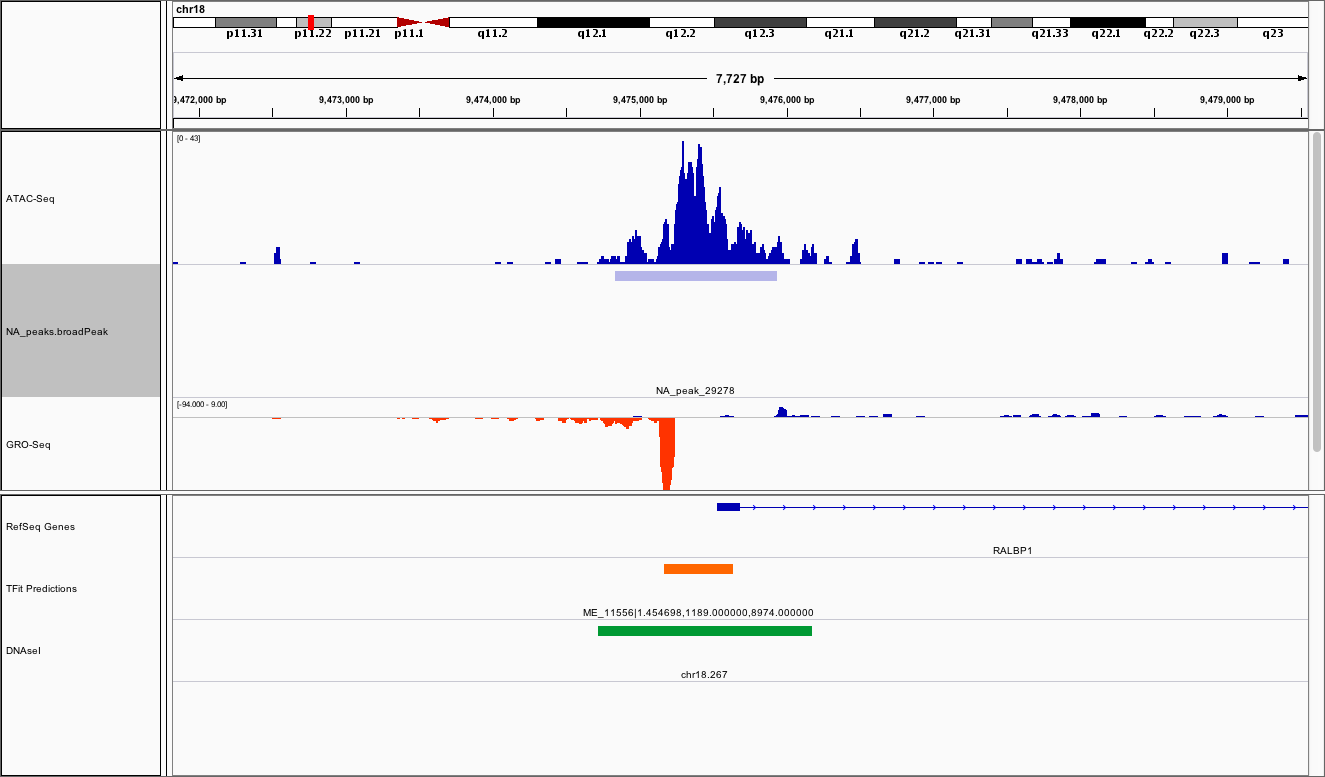
\includegraphics[width=\textwidth]{igvsnapshot}
  \label{igvsnapshot}
  \caption{A screenshot from IGV (Integrative Genomics Viewer \citep{igv})
    showing what an ATAC-Seq signal looks like (in blue top track), in the
    context of other assays, for a peak that overlaps an active gene enhancer
    site.  Other tracks depicted in the figure are:  ATAC-Seq peak boundaries obtained using
    MACS \citep{macs}, GRO-Seq signal (note that this nascent transcription
    assay is aware of DNA strand polarity, so this is a bidirectional signal),
    DNAse I \citep{dnase} signal (a different assay to inquire about chromatin
    accessiblity), and the reference genome annotations depicting gene location
  and their introns/exons.}
\end{figure}

\section{Background}
ATAC-Seq is a relatively new assay to obtain information from open chromatin
regions of the genome which excels in its simplicity, takes a total of three
hours to complete, and costs on the order of a few hundred dollars.  This makes
the assay highly desirable for inferring different kinds of information about
transcriptional activity, as most other assays that operate genome-wide and are
not focused to specific antibodies are over an order of magnitude more
expensive, take several days to complete, and have a higher error rate.  Thus,
utilizing ATAC-Seq data to classify different transcriptional conditions and
states is a worthwhile endeavor.

\section{Dataset}
Data files before processing are saved in the BED format.  These files can be
fed to a peak finding software which outputs the average region that is
considered a peak and generates a file which is similar to the BED format.  All
files will be aligned to the ``hg19'' human reference genome, and will
correspond to assays made using the same cell line (K562) and experimental
conditions.

The ATAC-Seq peaks represent approximate regions of the genome that are
accessible to transcription factors and other protiens involved in gene
regulation.  The size of the training data available, although it varies by
assay, is generally on the order of 80,000 peaks.

A TFit predictions file, also in the BED format, is generated from a software
tool developed at the Dowell Lab at the University of Colorado, Boulder.  This
tool identifies active regions based on GRO-Seq (Global Run-On
followed by sequencing \citep{gro}) data, an example of a longer, more sophisticated and
expensive assay.  These regions will be taken as our ground truth.  ATAC-Seq
peaks overlapping TFit regions will be considered ``active'' and ``inactive''
otherwise.  The ``overlap'' may be dependent on the biological context, and may
be expanded from a strict overlap to regions which are 1000 base-pairs from an
ATAC-Seq peak's median and 1000 base-pairs from the TFit region median overlap.

\begin{figure}[H]
  \centering
  \begin{subfigure}{0.25\textwidth}
    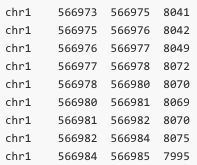
\includegraphics[width = \linewidth]{before_proc}
  \end{subfigure}%
  \hspace{10mm}%
  \begin{subfigure}{0.65\textwidth}
    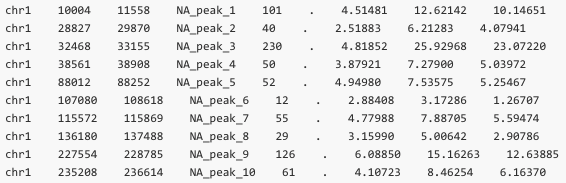
\includegraphics[width = \linewidth]{after_proc}
  \end{subfigure}
  \label{BED_DATA}
  \caption{\textbf{Left}: Example data file in the BED format.  The first column denotes
  the chromosome.  The second and third column denote the start and end of a
  sequence and the final column denotes sequencing depth.  \textbf{Right:}
  Example data file after processing to find peaks.  The first three columns
  are the same as in the unprocessed file, and the forth column denotes peak name.}
\end{figure}


\newpage
\section{Proposed Methods}
We propose three approaches to classifying these ATAC-Seq peaks.

\textbf{Feature Engineering} - Use domain knowledge to extract salient
  features from our dataset, which can be used with traditional supervised
  learning methods such as feed forward neural networks, SVMs, etc.  Some
  initial proposed features include:
  \begin{itemize}
  \item Peak width/height
  \item Distance between peaks (previous or next)
  \item Coefficients obtained from Fourier or wavelet transforms
  \end{itemize}

  \textbf{Peaks as Features} - We can treat the peaks as a time varying digital
  signal and use techniques that can take advantage of the temporal structure
  of our data.  Some proposed methods include:
  \begin{itemize}
  \item 1D convolutional and recurrent neural networks
  \item Hidden Markov Models
  \end{itemize}

  \textbf{Unsupervised Feature Learning} - Instead of hand picking features,
  use unsupervised methods to learn features from unlabeled input data which
  can then be used with supervised methods mentioned earlier.  Some proposed
  methods include:
  \begin{itemize}
  \item k-means clustering
  \item Autoencoders
  \item Principal Component Analysis
  \end{itemize}


\bibliographystyle{plain}
\bibliography{proposal}

\end{document}